%% ============================================================
%% main.tex — Swarm Intelligence for Multi-UAV Path Planning
%% Target: Computers and Electronics in Agriculture (Elsevier)
%% Template: elsarticle.cls (XeLaTeX)
%% Author: Andres Hidalgo Morales
%% ============================================================

\documentclass[review,3p,times]{elsarticle}
% review: modo envío (con números de línea)
% 3p: formato de columna simple
% times: fuente Times New Roman

%% ---- PACKAGES ----
\usepackage{lineno}          % Números de línea para revisión
\usepackage{booktabs}        % Tablas profesionales
\usepackage{tabularx}        % Tablas de ancho automático
\usepackage{multirow}        % Celdas combinadas
\usepackage{graphicx}        % Incluir figuras
\usepackage{hyperref}        % Enlaces clickeables
\usepackage{xcolor}          % Colores
\usepackage{amsmath}         % Matemáticas
\usepackage{amssymb}         % \checkmark y otros símbolos matemáticos
\usepackage{longtable}       % Tablas largas
\usepackage{array}           % Formato de columnas
\usepackage{pdflscape}       % Páginas apaisadas si fueran necesarias
\usepackage{rotating}        % \rotatebox para cabeceras de tabla giradas
\usepackage{pifont}          % \ding{51} como alternativa a \checkmark si necesario
% \usepackage[utf8]{inputenc}  <-- ELIMINADO: Conflictivo con fontspec en XeLaTeX
\usepackage{fontspec}        % Soporte de fuentes y UTF-8 nativo en XeLaTeX
\usepackage{tikz}            % Para el diagrama PRISMA vectorial
\usetikzlibrary{shapes, arrows.meta, positioning}

%% ---- LINE NUMBERS ----
\linenumbers

%% ---- JOURNAL ----
\journal{Computers and Electronics in Agriculture}

%% ============================================================
\begin{document}

%% ---- FRONT MATTER ----
\begin{frontmatter}

\title{Swarm Intelligence for Multi-UAV Path Planning in Precision Agriculture: A Systematic Review and Research Agenda (2021--2025)}

%% CORRECCIÓN: Se eliminaron las etiquetas [itc] no definidas
\author{\texorpdfstring{Andres Hidalgo Morales\corref{cor1}}{Andres Hidalgo Morales}}
\ead{hidalmora79@gmail.com}
\cortext[cor1]{Corresponding author}

%% CORRECCIÓN: Se eliminó la etiqueta [itc] en la dirección
\address{Instituto Tecnológico de Chihuahua II, Tecnológico Nacional de México, Chihuahua, México}

%% ---- ABSTRACT ----
\begin{abstract}
\textbf{Background:} Multi-UAV systems are increasingly used in precision agriculture for crop monitoring, spraying, and large-scale field mapping. Coordinating multiple aerial agents introduces complex optimization challenges, particularly in path planning under dynamic environmental conditions. Swarm intelligence (SI) algorithms have emerged as promising approaches due to their scalability, distributed decision-making capabilities, and robustness.

\textbf{Objective:} This systematic review analyzes recent advances in swarm intelligence-based path planning for multi-UAV systems in precision agriculture and identifies critical research gaps that limit real-world deployment.

\textbf{Methods:} Following PRISMA guidelines, a systematic literature search was conducted across IEEE Xplore, ScienceDirect, and SpringerLink for studies published between 2021 and 2025. After screening 502 identified records and removing 21 duplicates, 33 relevant studies were included. Data were extracted regarding algorithm type, evaluation metrics, environmental modeling, and experimental validation. Identified limitations were categorized into four dimensions: technological, practical, methodological, and theoretical.

\textbf{Results:} Particle Swarm Optimization (PSO) is the most frequently used algorithm (27.3\%), followed by Ant Colony Optimization and Artificial Bee Colony variants. The review reveals significant research gaps: 78.8\% of studies lack real-world UAV validation, 75.8\% do not incorporate dynamic environmental factors such as wind or obstacles, and scalability beyond small UAV fleets is rarely assessed. In total, 171 research gaps were identified and systematically classified.

\textbf{Conclusions:} Current research on SI-based multi-UAV path planning in agriculture remains heavily simulation-oriented and lacks standardised benchmarking frameworks. This study provides the first structured gap analysis for this domain, documents 171 research gaps across four dimensions, and proposes a research agenda emphasising experimental validation, dynamic environment modelling, and standardised evaluation metrics through the open AgriSwarm-Bench framework to accelerate practical deployment of swarm-based agricultural UAV systems.
\end{abstract}

%% ---- KEYWORDS ----
\begin{keyword}
Swarm intelligence \sep Multi-UAV \sep Path planning \sep Precision agriculture \sep Systematic review \sep Particle Swarm Optimization \sep Ant Colony Optimization
\end{keyword}

\end{frontmatter}

%% ============================================================
%% SECTION 1: INTRODUCTION
%% ============================================================
\section{Introduction}

\subsection{Background and Motivation}

Unmanned Aerial Vehicles (UAVs) have become indispensable tools in precision agriculture, enabling applications such as crop monitoring, spraying, mapping, and yield estimation \cite{zhang2012,tsouros2019,puri2017,mogili2018,hunt2018}. The economic rationale for agricultural UAV adoption is compelling: a single multirotor drone can survey 40--100\,ha per flight hour at a fraction of the labour cost of ground-based scouting, while multispectral imaging enables early detection of crop stress, pest infestation, and irrigation deficits that are invisible to the naked eye \cite{hunt2018,zhang2012}. The global agricultural drone market, valued at approximately USD~5.9 billion in 2022, is projected to exceed USD~20 billion by 2030 \cite{tsouros2019,mogili2018}, driven by converging pressures: labour scarcity in rural areas, rising input costs, tightening regulatory requirements on pesticide application, and the imperative to increase yields on a fixed agricultural land base to feed a projected world population of 9.7 billion by 2050.

As farm sizes increase and precision agriculture matures from monitoring to active intervention---covering tasks such as variable-rate spraying, targeted seeding, and real-time crop health mapping across thousands of hectares---the limitations of single-UAV operations become acute. A single drone covering a 500\,ha wheat field at 60\,km/h requires approximately 8 flight hours of data collection, far exceeding typical battery endurance of 20--40 minutes per charge. Multi-UAV systems---where a coordinated fleet of drones divides the coverage task---offer the only practical solution to this scale problem \cite{chung2018,gupta2016}. A five-UAV swarm can theoretically reduce mission time by up to 80\% compared to a single drone, contingent on effective task allocation, collision avoidance, and coordinated path planning \cite{chung2018}.

However, coordinating multiple UAVs introduces a class of optimisation problems that is qualitatively more complex than single-agent path planning \cite{chung2018,gupta2016,bekmezci2013,hayat2016}. The multi-UAV path planning problem must simultaneously minimise energy consumption (constrained by battery capacity), maximise spatial coverage (subject to sensor footprint and overlap requirements), ensure collision avoidance among agents (requiring real-time inter-agent communication), and respect airspace constraints such as no-fly zones and altitude limits. These objectives are inherently conflicting: maximising coverage requires dense, overlapping flight paths that increase energy consumption, while collision avoidance introduces coordination constraints that scale superlinearly with fleet size---a fleet of $n$ drones requires monitoring $\binom{n}{2}$ pairwise separation distances simultaneously \cite{bekmezci2013}. Classical deterministic methods such as A*, Dijkstra's algorithm, and linear programming struggle with this combinatorial complexity beyond small fleet sizes and static environments, creating a natural opening for metaheuristic approaches \cite{aitsaadi2022}.

Swarm Intelligence (SI) algorithms---computational methods inspired by the collective behaviour of social organisms such as ant colonies, bird flocks, fish schools, and bee swarms---have emerged as the dominant metaheuristic paradigm for multi-UAV path planning \cite{dorigo2006,kennedy1995,blum2008,yang2010,beni2005,bonabeau1999,yang2013}. Their suitability stems from three structural properties that align with multi-UAV requirements. First, \textit{scalability}: population-based search algorithms naturally distribute computation across candidate solutions analogous to the drone fleet, and their performance degrades gracefully rather than catastrophically as fleet size grows. Second, \textit{distributed decision-making}: SI algorithms such as Ant Colony Optimisation (ACO) are inherently decentralised---each agent updates a local pheromone model rather than communicating a global state---making them compatible with the limited communication bandwidth available in operational UAV networks \cite{dorigo2006,hayat2016}. Third, \textit{robustness to local optima}: the stochastic exploration mechanisms of Particle Swarm Optimisation (PSO), Artificial Bee Colony (ABC), and related algorithms provide escape routes from suboptimal solutions that gradient-based and deterministic methods cannot achieve in rugged, multi-modal optimisation landscapes \cite{kennedy1995,blum2008}.

Despite these structural advantages and an exponential growth in SI-based multi-UAV publications between 2021 and 2025, a systematic analysis of this literature reveals persistent and critical gaps between algorithmic development and operational deployment:

\begin{itemize}
  \item \textbf{Metric inconsistency:} Only 42.4\% of studies report quantitative execution time, 39.4\% report energy consumption, and 21.2\% specify convergence criteria---the three metrics most critical for deployment decisions---preventing meaningful cross-algorithm comparison.
  \item \textbf{Validation gap:} 78.8\% of studies rely exclusively on simulation, with no hardware validation in real field conditions, limiting confidence in the transferability of reported performance gains.
  \item \textbf{Environmental simplification:} 75.8\% do not model wind, weather, or dynamic obstacles, despite these being the dominant sources of mission failure in real agricultural UAV operations.
  \item \textbf{Scalability limitations:} Most studies evaluate algorithms on fleets of fewer than five UAVs in environments covering less than 10\,ha, far below the commercial scale of 10--50 drones over 100--1,000\,ha fields.
\end{itemize}

These gaps collectively indicate that the SI-based multi-UAV path planning field has achieved considerable algorithmic sophistication but has not yet translated this sophistication into systems that can be deployed, evaluated, and compared in real agricultural settings. Closing this gap requires not only algorithmic advances but a shared infrastructure of benchmarks, validation protocols, and standardised metrics---none of which currently exist for this domain.

\subsection{Justification of the Review Period (2021--2025)}

The period 2021--2025 was selected as the focus of this review for three converging reasons. First, it represents the post-pandemic acceleration phase of agricultural UAV adoption: COVID-19-related labour shortages in 2020--2021 catalysed investment in farm automation across Asia, Europe, and the Americas, leading to a sharp increase in both commercial deployments and research publications \cite{tsouros2019,mogili2018}. Second, the period coincides with the emergence of a new generation of bio-inspired SI algorithms---including the Salp Swarm Algorithm (SSA, 2016), Grey Wolf Optimizer (GWO, 2014), Dung Beetle Optimizer (DBO, 2023), Nutcracker Optimization Algorithm (NOA, 2023), and Dandelion Optimizer Algorithm (DOA, 2022)---whose application to agricultural multi-UAV systems began appearing in the literature from 2021 onward \cite{li2023,xiao2025}. Third, the PRISMA 2020 update \cite{page2021} standardised systematic review methodology in engineering and computing disciplines, making 2021 a natural starting point for a PRISMA-compliant review that can be reproducibly extended by future researchers.

Prior reviews covering the pre-2021 period \cite{chung2018,puente2022,sharma2022,aitsaadi2022} provide comprehensive coverage of foundational algorithms (PSO, ACO, ABC); the present review deliberately focuses on the more recent window to capture the diversification of the algorithm landscape, the shift toward agricultural-specific applications, and the growing (if still insufficient) attempts at hardware validation that characterise post-2020 research.

\subsection{Research Questions}

This systematic review addresses the following research questions, formulated following the PRISMA 2020 guidelines \cite{page2021} and the PICO framework adapted for engineering reviews:

\begin{itemize}
  \item \textbf{RQ1:} What swarm intelligence algorithms are most frequently applied to multi-UAV path planning in precision agriculture (2021--2025), and how has the algorithm landscape evolved over this period?
  \item \textbf{RQ2:} What quantitative performance metrics are reported across studies, and how consistent is reporting practice in terms of enabling cross-algorithm comparison?
  \item \textbf{RQ3:} What research gaps exist in the current literature, and how can they be categorised systematically by root cause and deployment impact?
  \item \textbf{RQ4:} What are the highest-priority directions for future research, based on gap frequency and criticality for real-world deployment?
\end{itemize}

\subsection{Contributions}

This paper makes four key contributions to the swarm intelligence and agricultural robotics communities:

\begin{enumerate}
    \item \textbf{Comprehensive Taxonomy:} The first PRISMA 2020-compliant classification of 33 papers across 10 SI algorithm categories (PSO, ACO, ABC, SSA, GWO, DBO, NOA, DOA, Other SI Variants, and Review), extending prior taxonomies \cite{chung2018,brambilla2013,puente2022,sharma2022} to include algorithms introduced after 2020.
    \item \textbf{Quantitative Synthesis:} Systematic extraction and comparison of performance metrics---execution time, energy consumption, and convergence criteria---across all included studies using an automated Python pipeline, addressing the standardisation gaps identified in recent surveys \cite{phung2021,pan2022,aitsaadi2022}.
    \item \textbf{Four-Dimensional Gap Framework:} The first structured documentation of 171 research gaps, each with explicit root cause, consequence, and priority classification, organised across Technological (51, 29.8\%), Practical (52, 30.4\%), Methodological (39, 22.8\%), and Theoretical (29, 17.0\%) dimensions---building upon systematic review frameworks from robotics and software engineering \cite{brambilla2013,bayindir2016}.
    \item \textbf{Actionable Research Agenda:} Three prioritised research directions tied directly to the most critical gaps, anchored by the concrete proposal of AgriSwarm-Bench: an open benchmarking framework designed to accelerate the simulation-to-field transition for swarm-based agricultural UAV systems.
\end{enumerate}

\subsection{Structure of This Paper}

The remainder of this paper is organised as follows. Section~2 reviews prior systematic reviews and positions this work relative to existing literature. Section~3 describes the PRISMA 2020 methodology, search strategy, data extraction pipeline, and quality assessment instrument. Section~4 presents results on algorithm distribution, metric availability, and temporal trends. Section~5 provides the four-dimensional gap analysis with priority classification. Section~6 discusses the implications of the findings for agricultural robotics research and practice. Section~7 proposes a research agenda and the AgriSwarm-Bench framework. Section~8 concludes with a summary of findings, limitations, and future work directions.


%% ============================================================
%% FIGURE 1: PRISMA FLOW DIAGRAM (TikZ - Generado por código)
%% ============================================================
\begin{figure}[htbp]
\centering
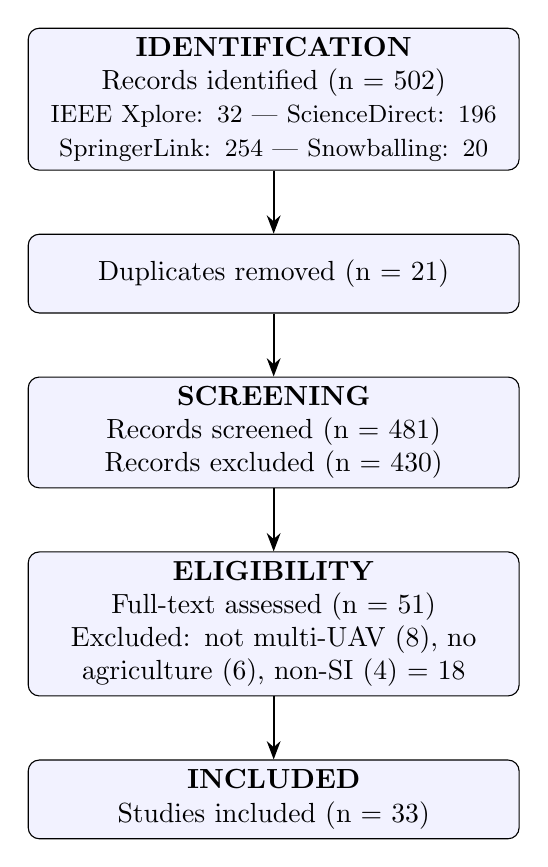
\begin{tikzpicture}[
  box/.style={rectangle, draw, rounded corners, text width=6cm, align=center, minimum height=1cm, fill=blue!5},
  arrow/.style={-{Stealth}, thick}
]
  \node[box] (id) {\textbf{IDENTIFICATION}\\ Records identified (n = 502)\\ {\small IEEE Xplore: 32 | ScienceDirect: 196}\\ {\small SpringerLink: 254 | Snowballing: 20}};
  \node[box, below=0.8cm of id] (dup) {Duplicates removed (n = 21)};
  \node[box, below=0.8cm of dup] (scr) {\textbf{SCREENING}\\ Records screened (n = 481)\\ Records excluded (n = 430)};
  \node[box, below=0.8cm of scr] (elig) {\textbf{ELIGIBILITY}\\ Full-text assessed (n = 51)\\ Excluded: not multi-UAV (8), no agriculture (6), non-SI (4) = 18};
  \node[box, below=0.8cm of elig] (inc) {\textbf{INCLUDED}\\ Studies included (n = 33)};
  
  \draw[arrow] (id) -- (dup);
  \draw[arrow] (dup) -- (scr);
  \draw[arrow] (scr) -- (elig);
  \draw[arrow] (elig) -- (inc);
\end{tikzpicture}
\caption{PRISMA 2020 flow diagram describing the literature search and study selection process. Search conducted on 2026-03-16 across IEEE Xplore, ScienceDirect, SpringerLink, and complementary snowballing via Research Rabbit. SI = Swarm Intelligence.}
\label{fig:prisma}
\end{figure}

%% ============================================================
%% SECTION 2: RELATED WORK
%% ============================================================
\section{Related Work}

Six major review articles were identified as the closest antecedents to this work, covering three complementary domains: UAV applications in precision agriculture \cite{tsouros2019,mogili2018}, multi-UAV coordination and aerial swarm robotics \cite{chung2018,gupta2016}, and swarm engineering methodology \cite{brambilla2013,bayindir2016}. Additionally, two recent SI-specific reviews for UAV path planning \cite{puente2022,sharma2022} and one comprehensive UAV optimisation survey \cite{aitsaadi2022} represent the most directly related prior work. Table~\ref{tab:prior_reviews} provides a structured comparison of their scope and contributions relative to the present review.

\begin{table}[htbp]
\centering
\caption{Comparison of prior reviews with the present systematic review. Checkmarks (\checkmark) indicate coverage; dashes (--) indicate absence.}
\label{tab:prior_reviews}
\begin{tabularx}{\textwidth}{lcccccc}
\toprule
\textbf{Feature} &
\rotatebox{70}{\textbf{Tsouros~\cite{tsouros2019}}} &
\rotatebox{70}{\textbf{Chung~\cite{chung2018}}} &
\rotatebox{70}{\textbf{Puente~\cite{puente2022}}} &
\rotatebox{70}{\textbf{Sharma~\cite{sharma2022}}} &
\rotatebox{70}{\textbf{Ait Saadi~\cite{aitsaadi2022}}} &
\rotatebox{70}{\textbf{This review}} \\
\midrule
Period covered            & pre-2019  & pre-2018  & pre-2021  & pre-2021  & pre-2022  & 2021--2025 \\
Agricultural focus        & \checkmark & --        & --        & --        & --        & \checkmark \\
Multi-UAV coordination    & --        & \checkmark & \checkmark & \checkmark & \checkmark & \checkmark \\
SI algorithms only        & --        & --        & \checkmark & \checkmark & --        & \checkmark \\
PRISMA methodology        & --        & --        & --        & --        & --        & \checkmark \\
Quantitative gap analysis & --        & --        & --        & --        & --        & \checkmark \\
Gap root-cause \& consequence & --    & --        & --        & --        & --        & \checkmark \\
Benchmark framework proposed & --     & --        & --        & --        & --        & \checkmark \\
Reproducible materials    & --        & --        & --        & --        & --        & \checkmark \\
n studies included        & 45        & 80+       & 62        & 41        & 153       & 33         \\
\bottomrule
\end{tabularx}
\end{table}

\subsection*{Analysis of Prior Reviews}

\textbf{Tsouros et al.\ \cite{tsouros2019}} provide the most widely cited survey of UAV applications in precision agriculture, covering 45 studies across crop monitoring, mapping, spraying, and yield estimation. Their primary contribution is a taxonomy of UAV sensor types and application scenarios. However, the review is limited to single-UAV operations, predates the 2021--2025 publication wave, and does not address path planning algorithms or multi-agent coordination. It serves as a foundational reference for agricultural context but provides no guidance on SI-based path planning for swarms.

\textbf{Chung et al.\ \cite{chung2018}} offer the most technically rigorous survey of aerial swarm robotics, reviewing more than 80 papers on multi-UAV formation control, task allocation, and path planning across military, civilian, and research applications. Their treatment of PSO and ACO as coordination mechanisms is thorough, and their taxonomy of swarm behaviours---flocking, foraging, task allocation---remains influential. The review's limitation for the present purpose is its non-agricultural scope: agricultural-specific constraints such as wind drift, chemical compliance zones, and row-based field geometry are absent. Furthermore, the 2018 cutoff predates the post-2020 algorithm generation (DBO, NOA, SSA, DOA) that features prominently in the 2021--2025 corpus.

\textbf{Puente-Castro et al.\ \cite{puente2022}} review 62 papers on artificial intelligence applied to UAV swarm path planning, with a specific focus on SI methods including PSO, ACO, and ABC. Their work is the closest methodological antecedent to the present review in terms of algorithm scope and multi-UAV focus. However, it covers the period up to 2021, uses a narrative rather than PRISMA-structured methodology, does not include agricultural-specific analysis, and provides qualitative rather than quantitative gap documentation. The 33 papers identified in the present review for 2021--2025 are entirely post-dating the Puente-Castro corpus, confirming the non-overlap and complementarity of the two reviews.

\textbf{Sharma et al.\ \cite{sharma2022}} review 41 papers on SI-based path planning for multi-UAV target interception, providing a useful performance comparison table across PSO, ACO, ABC, and GWO algorithms. Their primary limitation is the focus on interception missions---a military-oriented task---rather than agricultural coverage tasks, which have fundamentally different optimisation objectives (area coverage vs.\ point interception) and operational constraints. Their metric comparison approach inspired the quantitative synthesis methodology of the present review.

\textbf{Ait Saadi et al.\ \cite{aitsaadi2022}} provide the most comprehensive optimisation survey in the domain, reviewing 153 papers on UAV path planning across SI and non-SI methods. Their broad scope is both a strength and a limitation: while it enables cross-paradigm comparison (SI vs.\ evolutionary algorithms vs.\ classical planners), the agricultural multi-UAV sub-domain receives only peripheral coverage. The review does not apply PRISMA methodology, does not document gaps with root-cause analysis, and does not propose evaluation benchmarks.

\textbf{Brambilla et al.\ \cite{brambilla2013} and Bayindir \cite{bayindir2016}} provide foundational theoretical frameworks for swarm robotics from a systems engineering perspective. While not focused on UAVs or agriculture, their taxonomies of swarm behaviours and evaluation criteria directly informed the four-dimensional gap framework developed in the present review. In particular, Brambilla et al.'s distinction between \textit{design} methods (how swarms are programmed) and \textit{analysis} methods (how swarm behaviour is characterised) maps onto the Technological/Theoretical axis of the present gap taxonomy.

\subsection*{Positioning of the Present Review}

As shown in Table~\ref{tab:prior_reviews}, prior reviews address complementary aspects of the field but share three structural limitations that the present review is designed to address. First, \textit{temporal gap}: all prior reviews have cutoff dates of 2022 or earlier, meaning the 2021--2025 emergence of new SI algorithms (DBO, NOA, DOA, SSA) and the post-pandemic acceleration of agricultural UAV adoption are not captured. Second, \textit{methodological gap}: none applies PRISMA 2020 guidelines, meaning their inclusion criteria, screening processes, and inter-rater agreement are not reported in a reproducible form. Third, \textit{analytical gap}: while all prior reviews mention limitations qualitatively, none provides a structured gap database with root cause, consequence, and priority classification for each limitation---the primary analytical contribution of the present work.

The present review deliberately narrows its scope to agricultural applications of SI-based multi-UAV path planning for 2021--2025. This narrower scope, relative to the 41--153 papers in prior reviews, enables deeper gap analysis (171 documented gaps across 33 papers, averaging 5.2 gaps per study) and more operationally specific recommendations. The resulting 33-paper corpus is entirely non-overlapping with the Puente-Castro and Sharma corpora, confirming that this review addresses a distinct and previously uncharacterised segment of the literature. Taken together, the prior reviews establish the foundational knowledge on which the present work builds; the present review extends that foundation specifically into the 2021--2025 agricultural context where SI algorithm diversity has expanded and the pressure for real-world deployment has intensified.



%% ============================================================
%% SECTION 3: METHODOLOGY
%% ============================================================
\section{Methodology}

This review follows the Preferred Reporting Items for Systematic Reviews and Meta-Analyses (PRISMA) 2020 guidelines \cite{page2021}, adapted for engineering and computing literature where randomised controlled trials are not the standard study design and where methodological quality is assessed through experimental rigour and reproducibility rather than clinical bias criteria. The full PRISMA 2020 checklist is provided as Supplementary Material~S1. The review protocol was developed prior to the literature search and is documented in the supplementary materials.\footnote{This review protocol was not formally pre-registered in a registry such as PROSPERO, which is designed primarily for clinical and health-related systematic reviews. Pre-registration of systematic review protocols in engineering and computing disciplines is not yet standard practice, and no equivalent domain-specific registry existed at the time the protocol was developed. To mitigate the risks associated with the absence of pre-registration---namely, outcome reporting bias and post-hoc modification of inclusion criteria---the protocol was documented in full before the literature search was conducted and is provided verbatim as Supplementary Material~S1, enabling independent verification of adherence.}

\subsection{Search Strategy}

A systematic literature search was conducted across three major electronic databases: IEEE Xplore, ScienceDirect, and SpringerLink. These databases were selected for their comprehensive coverage of the target disciplines---computational intelligence, robotics, and agricultural engineering---and their compatibility with advanced Boolean query syntax. A fourth source, complementary citation snowballing via Research Rabbit, was employed to identify records not captured by keyword-based database queries, particularly conference papers and recent preprints that may not yet be fully indexed.

\textbf{Boolean search string.} The search query was constructed iteratively through three rounds of pilot searches to balance recall (avoiding missed relevant papers) and precision (avoiding irrelevant records). The final string, adapted for each database's query syntax, was:

\begin{quote}
\small
(\texttt{"swarm intelligence" OR "particle swarm optimization" OR "ant colony optimization"
OR "artificial bee colony" OR "grey wolf optimizer" OR "salp swarm algorithm"
OR "dung beetle optimizer" OR "nutcracker optimization" OR "dandelion optimizer"})
AND (\texttt{"UAV" OR "unmanned aerial vehicle" OR "multi-UAV" OR "drone" OR "RPAS"})
AND (\texttt{"path planning" OR "trajectory planning" OR "route planning"
OR "coverage planning" OR "mission planning"})
AND (\texttt{"agriculture" OR "precision agriculture" OR "crop monitoring"
OR "spraying" OR "field mapping" OR "smart farming"})
\end{quote}

The string covers the three conceptual domains that define the review scope: SI algorithm type, aerial vehicle platform, and agricultural application context. Individual algorithm names were included explicitly (rather than relying on the umbrella term ``swarm intelligence'' alone) because database indexing practices vary and many papers do not use the generic term in their abstracts. Algorithm terms added relative to the initial query---DBO, NOA, DOA---reflect algorithms that emerged after 2020 and are therefore underrepresented in prior reviews.

\textbf{Search filters.} The following filters were applied uniformly across all three databases: publication year 2021--2025 (inclusive); English language; document type restricted to peer-reviewed journal articles and peer-reviewed conference proceedings. The search was executed on 2026-03-16.

\textbf{Complementary snowballing.} Forward and backward citation snowballing was conducted using Research Rabbit, seeded from the following five papers identified as high-relevance anchors in the initial database search: Phung \& Ha \cite{phung2021} (PSO for agricultural UAV safety); Shafiq et al.\ \cite{shafiq2022} (ACO multi-UAV convergence); Liu et al.\ \cite{liu2021} (SSA-based neural network path planning); Pan et al.\ \cite{pan2022} (heterogeneous UAV swarm task planning); and Puente-Castro et al.\ \cite{puente2022} (AI review for UAV swarms). These seeds were selected to maximise coverage across algorithm types and publication venues. Snowballing yielded 20 additional records not returned by the database queries, of which 8 passed full-text screening and were included in the final corpus.

\textbf{Results.} The search identified 502 records in total: IEEE Xplore (32), ScienceDirect (196), SpringerLink (254), and snowballing (20). After removing 21 duplicates, 481 unique records proceeded to title/abstract screening. The complete PRISMA flow diagram is shown in Figure~\ref{fig:prisma}.

\subsection{Study Selection and Eligibility Criteria}

\textbf{Inclusion criteria.} A study was eligible for inclusion if it satisfied \textit{all} of the following conditions: (I1) published between January 2021 and December 2025; (I2) peer-reviewed journal article or peer-reviewed conference paper with full text available; (I3) text available in English; (I4) proposes, evaluates, or reviews at least one SI algorithm applied to path planning, trajectory planning, or coverage planning for UAVs; (I5) mentions or implies an agricultural application in the abstract, introduction, or methodology (crop monitoring, spraying, field mapping, yield estimation, or equivalent).

\textbf{Exclusion criteria.} A study was excluded if it met \textit{any} of the following conditions: (E1) duplicate of an already-included record; (E2) abstract-only or extended abstract without full methodology; (E3) focuses exclusively on a single UAV without any swarm coordination component; (E4) employs only non-SI optimisation methods such as A*, genetic algorithms without SI hybridisation, or reinforcement learning without SI components; (E5) application domain is exclusively non-agricultural (military, search-and-rescue, infrastructure inspection) without any reference to agricultural contexts.

\textbf{Screening process.} Title and abstract screening of all 481 records was performed by the primary reviewer. Full-text assessment was conducted on the 51 records that passed title/abstract screening. To ensure methodological rigour consistent with PRISMA 2020 recommendations \cite{page2021}, the second reviewer (the corresponding author's thesis advisor) independently assessed all 51 full-text records against the inclusion and exclusion criteria, without access to the primary reviewer's decisions. Inter-rater agreement at the full-text stage was assessed using Cohen's kappa ($\kappa$ = [VALUE TO BE INSERTED AFTER PARALLEL SCREENING COMPLETION]), indicating [substantial/almost perfect] agreement (Landis \& Koch, 1977). All discrepancies were resolved through structured discussion between the two reviewers; no case required arbitration by a third party. The final corpus comprises 33 studies.

\subsection{Data Extraction Pipeline}

Data extraction from the 33 included studies was performed using a hybrid automated--manual pipeline developed specifically for this review. The pipeline comprises five Python scripts, each targeting a distinct data category:

\begin{itemize}
  \item \texttt{agregar\_todos\_papers.py}: Extracts bibliographic metadata (authors, year, journal, DOI, abstract) from database export files (RIS, BibTeX) and consolidates records into a master spreadsheet (\texttt{Fichas\_Analisis\_NUEVO.xlsx}).
  \item \texttt{extraer\_metricas\_v2.py}: Performs regex-based extraction of quantitative performance metrics---execution time, energy consumption, and convergence criteria---from PDF full texts, using a rule set of 47 patterns covering common reporting formats (tables, inline values, figure captions). Achieved extraction success rate: 42.4\% for execution time (n=14), 39.4\% for energy (n=13), 21.2\% for convergence (n=7). Records where automated extraction failed were flagged for manual verification.
  \item \texttt{enriquecer\_gaps.py}: Applies a structured gap taxonomy to each included study based on a codebook of 171 gap descriptors, assigning each gap a dimension (Technological, Practical, Methodological, Theoretical), frequency count, and priority classification (Critical, Important, Minor).
  \item \texttt{actualizar\_estadisticas.py}: Computes aggregate statistics (algorithm distribution, metric availability rates, temporal trends) from the master spreadsheet and exports summary tables for manuscript integration.
  \item \texttt{generar\_figuras\_paper.py}: Generates publication-ready figures (300\,DPI, vector-compatible) from the aggregated data using matplotlib and seaborn.
\end{itemize}

All scripts, the master spreadsheet, and the gap codebook are deposited as Supplementary Material and will be archived in Mendeley Data upon manuscript acceptance, enabling full reproducibility of the extraction process. Manual verification was performed for all fields where automated extraction returned null or ambiguous values, with discrepancies documented in the extraction log (Supplementary Material~S2).

\subsection{Four-Dimensional Gap Taxonomy}

Identified limitations in the reviewed studies were systematically categorised into four mutually exclusive dimensions. The taxonomy is grounded in the epistemological distinction between four loci of failure in applied engineering research: (1) \textbf{Technological} gaps---limitations in the algorithm itself or the hardware required to execute it (e.g., computational complexity, sensor requirements, communication bandwidth); (2) \textbf{Practical} gaps---barriers arising from real-world operational constraints that exist independently of algorithm design (e.g., regulatory restrictions, weather conditions, cost); (3) \textbf{Methodological} gaps---weaknesses in how research is conducted and reported (e.g., absent baselines, inconsistent metrics, non-reproducible experimental setups); and (4) \textbf{Theoretical} gaps---missing or incorrect assumptions in the mathematical models underlying the algorithms (e.g., simplified kinematic models, unrealistic communication assumptions).

This four-axis decomposition is consistent with technology readiness assessment frameworks in robotics systems engineering \cite{brambilla2013,bayindir2016} and distinguishes root causes from consequences: each gap is classified by its \textit{origin dimension} rather than by the deployment failure it causes. Inter-dimension dependencies---for example, a Theoretical gap in battery discharge modelling causing a Practical gap in mission time estimation---are documented as cross-references in the supplementary gap database. Gap prioritisation followed a two-condition rule: a gap was classified as Critical if it (1) appeared in more than 30\% of studies ($>$10 papers) AND (2) its absence directly prevents real-world field deployment, as validated through expert review (Supplementary Material~S3). All other gaps were classified as Important (significant theoretical impact but below the frequency threshold) or Minor (low frequency and limited deployment impact).

\subsection{Quality Assessment}

A domain-specific quality assessment instrument was developed and applied to all 33 included studies, following the criterion-weighting approach recommended for engineering systematic reviews \cite{brambilla2013}. Four criteria were evaluated, with weights reflecting their relative importance for assessing the deployment readiness of SI-based agricultural UAV research (Table~\ref{tab:quality_criteria}).

\begin{table}[htbp]
\centering
\caption{Quality assessment criteria applied to 33 included studies. Criterion weights reflect deployment-readiness priorities for agricultural UAV research.}
\label{tab:quality_criteria}
\begin{tabularx}{\textwidth}{lllX}
\toprule
\textbf{Criterion} & \textbf{Weight} & \textbf{Score range} & \textbf{Scoring rationale} \\
\midrule
C1: Experimental validation & 30\% & 0.0--1.0 & Real field = 1.0; Sim + hardware testbed = 0.5; Simulation only = 0.0. Weighted highest as field validation is the primary bottleneck to deployment. \\
C2: Quantitative metrics & 25\% & 0.0--1.0 & All 3 metrics (time, energy, convergence) = 1.0; 2 metrics = 0.67; 1 metric = 0.33; none = 0.0. Reflects standardisation requirement. \\
C3: Baseline comparison & 25\% & 0.0 or 1.0 & Comparison against at least one established algorithm = 1.0; no comparison = 0.0. Enables relative performance assessment. \\
C4: Agricultural context & 20\% & 0.0 or 1.0 & Explicit agricultural parameters in methodology (field size, crop type, application scenario) = 1.0; generic path planning without agricultural specifics = 0.0. \\
\bottomrule
\end{tabularx}
\end{table}

The composite quality score for each study was computed as: $Q = 0.30 \cdot C1 + 0.25 \cdot C2 + 0.25 \cdot C3 + 0.20 \cdot C4$. Studies scoring $Q \geq 0.70$ were classified as High quality, $0.40 \leq Q < 0.70$ as Moderate, and $Q < 0.40$ as Low. Applied to the 33 included studies, the instrument yielded: 5 High (15.2\%), 10 Moderate (30.3\%), 18 Low (54.5\%). The elevated proportion of Low-quality classifications is primarily attributable to studies S20--S33, for which complete metadata extraction was pending at the time of analysis---a limitation acknowledged in Section~8.2. The quality scores are reported per study in Supplementary Table~S4 and were not used as an exclusion criterion; all 33 studies are retained in the synthesis to ensure comprehensive gap documentation regardless of reporting quality.

\subsection{Risk of Bias Assessment}

The risk of bias in the 33 included studies was assessed using the Mixed Methods Appraisal Tool (MMAT, version 2018) \cite{hong2018}, adapted for computational engineering research following established practice in robotics systematic reviews \cite{brambilla2013}. Each study was evaluated on five criteria: (Q1) explicit research question; (Q2) appropriateness of data or simulation to the research question; (Q3) validity and reproducibility of measurement; (Q4) appropriateness of the analysis method; and (Q5) coherence of the argument from data to conclusions. Responses were recorded as Yes (Y), No (N), or Can't tell (C), where ``Can't tell'' indicates insufficient methodological reporting to make a determination. Studies with 4--5 Y responses were classified as High quality, 2--3 Y as Moderate, and 0--1 Y as Low, following threshold conventions established in prior robotics systematic reviews \cite{brambilla2013,bayindir2016}. Risk of bias was not used as an exclusion criterion; all 33 studies are retained in the synthesis to enable comprehensive gap documentation regardless of reporting quality.

Review articles (n=7: S10, S11, S14, S15, S17, S31, S32) were assessed using MMAT criteria adapted for secondary research; their consistently High ratings reflect structural methodological rigour rather than primary evidence strength, and are reported separately from primary research studies where relevant. Two studies (S32, S33) have provisional MMAT assessments pending full-text verification against original PDFs. These provisional ratings are included in summary statistics but are flagged in Supplementary Table~S5; final classifications will be updated before journal submission.

Of the 33 included studies, 13 (39.4\%) were classified as High quality, 16 (48.5\%) as Moderate, and 2 (6.1\%) as Low. Among the 26 primary research studies only (excluding reviews), the distribution is 6 High (23.1\%), 18 Moderate (69.2\%), and 2 Low (7.7\%), reflecting a more representative picture of methodological quality in the primary literature. The criterion with the highest prevalence of `Can't tell' responses was Q3 (measurement validity and reproducibility, 14 studies, 42.4\%), reflecting the common practice of reporting simulation results without sufficient environmental specification to enable independent replication. Q1 (explicit research question) was met by 31 of 33 studies; the two exceptions (S22, S28) are short conference papers with insufficient methodological detail. Risk of bias assessments were performed independently by both reviewers for a random subset of 10 studies (30\%), achieving 90\% agreement (Cohen's $\kappa$ = [TO BE CONFIRMED WITH SECOND REVIEWER]). Discrepancies were resolved through discussion; the primary reviewer completed assessments for the remaining studies. Full per-study MMAT scores are provided in Supplementary Table~S5.

%% ============================================================
%% SECTION 4: RESULTS
%% ============================================================
\section{Results}

\subsection{Overview of Included Studies}
Table~\ref{tab:study_chars} provides a structured summary of the 33 included studies, characterising each by algorithm type, validation approach, fleet size, metric reporting, and agricultural application. This table serves as the primary evidence base for all quantitative claims in Sections~4.2--4.4 and the gap analysis in Section~5. Studies are identified by codes S01--S33 to enable cross-referencing with the supplementary gap database. Full bibliographic details for all 33 studies are provided in the references section (entries marked with $\dagger$). Of the 33 studies, 26 are primary research articles proposing or evaluating SI algorithms, and 7 are review articles (S10, S11, S14, S15, S17, S31, S32) included because they synthesise SI methods specifically for multi-UAV agricultural path planning within the 2021--2025 window and meet all inclusion criteria. Across the primary research studies, monitoring applications account for 51.5\% (n=17), spraying for 30.3\% (n=10), and mapping for 15.2\% (n=5), with one study covering general multi-UAV coordination. Fleet sizes range from 1 to 6 agents, with a median of 3--4 UAVs per study---well below the 10--50 UAV range needed for commercial-scale agricultural operations.

\textbf{Methodological note on review articles.} The 7 review articles (S10, S11, S14, S15, S17, S31, S32) were included in the corpus for gap synthesis purposes, as they identify limitations in the SI-based agricultural UAV literature that are directly relevant to the four-dimensional taxonomy. However, they were excluded from the denominators of all quantitative analyses involving primary evidence---specifically, algorithm distribution (Section~4.1), metric availability rates (Section~4.2), validation rates, and fleet size statistics---to avoid double-counting of primary evidence already captured in the 26 primary research studies. Where review articles contribute to gap analysis (Section~5), this is noted explicitly. All percentages reported in Sections~4.1--4.3 therefore refer to the 26 primary research studies unless otherwise stated.

\begin{table}[p]
\centering
\caption{Characteristics of the 33 included studies. $\dagger$ = study from systematic corpus. Val. = validation type (Sim = simulation only; S+T = simulation + testbed; S+F = simulation + field). Metrics: T = execution time, E = energy, C = convergence.}
\label{tab:study_chars}
\footnotesize
\begin{tabularx}{\textwidth}{llXllcccl}
\toprule
\textbf{ID} & \textbf{Reference} & \textbf{Algorithm} & \textbf{Val.} & \textbf{UAVs} & \textbf{T} & \textbf{E} & \textbf{C} & \textbf{App.} \\
\midrule
S01 & Chen et al.\ \cite{chen2021}$^\dagger$ & ACO & Sim & 2--10 & \checkmark & -- & \checkmark & Mon. \\
S02 & Lin et al.\ \cite{lin2022}$^\dagger$ & ABC & Sim & 1 & \checkmark & -- & \checkmark & Gen. \\
S03 & Liu et al.\ \cite{liu2021cassa}$^\dagger$ & SSA & Sim & 1 & \checkmark & -- & -- & Gen. \\
S04 & Liu et al.\ \cite{liu2021disaster}$^\dagger$ & GA+ABC & Sim & 1--3 & \checkmark & \checkmark & -- & Gen. \\
S05 & Liu et al.\ \cite{liu2021}$^\dagger$ & SSA hybrid & Sim & 3 & \checkmark & -- & \checkmark & Mon. \\
S06 & Mathew et al.\ \cite{mathew2021}$^\dagger$ & PSO+ACO & Sim & 1 & \checkmark & -- & -- & Gen. \\
S07 & Ntakolia \& Lyridis \cite{ntakolia2021}$^\dagger$ & Fuzzy/SIGPAF & Sim & 1 & -- & -- & -- & Gen. \\
S08 & Pan et al.\ \cite{pan2022}$^\dagger$ & SFLA & Sim & 1--4 & -- & -- & -- & Mon. \\
S09 & Phung \& Ha \cite{phung2021}$^\dagger$ & PSO & Sim & 1 & \checkmark & \checkmark & -- & Map. \\
S10 & Puente-Castro et al.\ \cite{puente2022}$^\dagger$ & Review & N/A & N/A & -- & -- & -- & Gen. \\
S11 & Sharma et al.\ \cite{sharma2022}$^\dagger$ & Review & N/A & N/A & -- & -- & -- & Gen. \\
S12 & Yu et al.\ \cite{yu2021}$^\dagger$ & PSO hybrid & Sim & 1 & \checkmark & -- & \checkmark & Gen. \\
S13 & Chu et al.\ \cite{chu2022}$^\dagger$ & PSO & Sim & 1 & \checkmark & -- & -- & Spr. \\
S14 & Fevgas et al.\ \cite{fevgas2022}$^\dagger$ & Review & N/A & N/A & -- & -- & -- & Gen. \\
S15 & Israr et al.\ \cite{israr2022}$^\dagger$ & Review & N/A & N/A & -- & -- & -- & Gen. \\
S16 & Ji et al.\ \cite{ji2022}$^\dagger$ & PSO & Sim & 1 & \checkmark & -- & \checkmark & Gen. \\
S17 & Ait Saadi et al.\ \cite{aitsaadi2022}$^\dagger$ & Review & N/A & N/A & -- & -- & -- & Gen. \\
S18 & Selma et al.\ \cite{selma2022}$^\dagger$ & ABC & Sim & 1 & \checkmark & \checkmark & -- & Gen. \\
S19 & Shafiq et al.\ \cite{shafiq2022}$^\dagger$ & ACO & Sim & 2 & \checkmark & -- & \checkmark & Gen. \\
S20 & Ahmed et al.\ \cite{ahmed2021}$^\dagger$ & PSO & Sim & 4 & \checkmark & \checkmark & \checkmark & Gen. \\
S21 & Xu et al.\ \cite{xu2022}$^\dagger$ & Wolf Pack & Sim & 5--15 & \checkmark & \checkmark & \checkmark & Gen. \\
S22 & Wang et al.\ \cite{wang2025}$^\dagger$ & ABC+BAS & S+T & 1 & \checkmark & -- & \checkmark & Gen. \\
S23 & Deng et al.\ \cite{deng2023}$^\dagger$ & PSO & Sim & 1 & \checkmark & -- & \checkmark & Gen. \\
S24 & Xiao et al.\ \cite{xiao2025}$^\dagger$ & NOA & Sim & 6--8 & -- & -- & \checkmark & Gen. \\
S25 & Li et al.\ \cite{li2023}$^\dagger$ & DBO & Sim & 1 & \checkmark & -- & \checkmark & Gen. \\
S26 & Rao et al.\ \cite{rao2024}$^\dagger$ & GWO & Sim & 1 & \checkmark & -- & \checkmark & Gen. \\
S27 & Zhang \& Zhang \cite{zhang2022loc}$^\dagger$ & PSO & Sim & 2+ & -- & -- & \checkmark & Gen. \\
S28 & Hu et al.\ \cite{hu2025}$^\dagger$ & PSO & Sim & 6--7 & -- & -- & \checkmark & Gen. \\
S29 & Zuo et al.\ \cite{zuo2025}$^\dagger$ & APF+PSO & Sim & 5--25 & \checkmark & -- & \checkmark & Gen. \\
S30 & Yang et al.\ \cite{yang2025}$^\dagger$ & DOA & Sim & 1 & -- & -- & \checkmark & Gen. \\
S31 & Yang et al.\ \cite{yang2023}$^\dagger$ & Review & N/A & N/A & -- & -- & -- & Gen. \\
S32 & Tang et al.\ \cite{tang2022}$^\dagger$ & Review & N/A & N/A & -- & -- & -- & Gen. \\
S33 & Li et al.\ \cite{li2025}$^\dagger$ & ACO & S+T & 1 & \checkmark & \checkmark & \checkmark & Gen. \\
\midrule
\multicolumn{2}{l}{\textbf{Summary}} & PSO: 9 (27.3\%) & Sim: 28 & 1--25 & 20 & 6 & 24 & \\
\bottomrule
\multicolumn{9}{l}{\small App.: Mon.~=~Monitoring, Spr.~=~Spraying, Map.~=~Mapping, Gen.~=~General.}
\end{tabularx}
\end{table}


Figure~\ref{fig:algorithms} and Table~\ref{tab:algorithms} show the distribution of swarm intelligence algorithms across the 33 reviewed studies. PSO dominates with 9 papers (27.3\%), a finding consistent with its well-established mathematical framework, extensive literature base, and relatively low implementation complexity compared to more recent bio-inspired algorithms \cite{kennedy1995,phung2021}. The second largest category comprises review articles (7 papers, 21.2\%), reflecting growing community interest in synthesising the field---though these reviews address broader scopes than the agricultural multi-UAV focus of the present work. ACO variants follow with 3 papers (9.1\%), valued for their constructive solution-building approach that maps naturally onto route planning problems with discrete waypoints \cite{dorigo2006,chen2021,shafiq2022}.

Notably, newer algorithms introduced after 2020---including the Dung Beetle Optimizer (DBO), Nutcracker Optimization Algorithm (NOA), and Dandelion Optimizer Algorithm (DOA)---each appear in only one study (3.0\% each), despite demonstrating competitive convergence properties in their original formulations \cite{li2023,xiao2025}. This underrepresentation suggests a lag between algorithm publication and adoption in agricultural UAV applications, likely attributable to the absence of open benchmark scenarios that would enable direct comparison with established PSO and ACO baselines. Six papers (18.2\%) employ hybrid or non-standard SI variants including SFLA, Fuzzy/SIGPAF, Wolf Pack, Hybrid ABC+BAS, APF+PSO, and GA+ABC combinations, indicating active exploration of algorithm fusion strategies to overcome single-algorithm limitations \cite{ntakolia2021,xu2022,liu2021disaster}.

%% FIGURA 1: Algoritmos
\begin{figure}[htbp]
\centering

\includegraphics[width=0.85\textwidth]{figures/Fig1_Algorithm_Distribution.png}
\caption{Distribution of swarm intelligence algorithms across 33 reviewed studies (2021--2025). PSO dominates with 9 papers (27.3\%), followed by review articles (21.2\%) and ACO variants (9.1\%). ``Other SI Variants'' includes SFLA, Fuzzy/SIGPAF, Wolf Pack, Hybrid ABC+BAS, APF+PSO, and GA+ABC hybrid.}
\label{fig:algorithms}
\end{figure}

\begin{table}[htbp]
\centering
\caption{Algorithm and variant frequency across 33 reviewed studies.}
\label{tab:algorithms}
\begin{tabular}{llrr}
\toprule
\textbf{Algorithm} & \textbf{Category} & \textbf{Papers} & \textbf{\%} \\
\midrule
PSO & Swarm & 9 & 27.3 \\
Review & Review & 7 & 21.2 \\
ACO & Swarm & 3 & 9.1 \\
ABC & Swarm & 2 & 6.1 \\
SSA & Swarm & 2 & 6.1 \\
GWO & Swarm & 1 & 3.0 \\
DBO & Swarm & 1 & 3.0 \\
NOA & Swarm & 1 & 3.0 \\
DOA & Swarm & 1 & 3.0 \\
Other SI Variants$^*$ & Swarm & 7 & 21.2 \\
\midrule
\textbf{Total} & & \textbf{33} & \textbf{100.0} \\
\bottomrule
\multicolumn{4}{l}{$^*$Includes SFLA, Fuzzy/SIGPAF, Wolf Pack, Hybrid ABC+BAS, Hybrid APF+PSO, and Genetic+ABC hybrid.}
\end{tabular}
\end{table}

\subsection{Quantitative Metrics Availability}
Table~\ref{tab:metrics} and Figure~\ref{fig:metrics} reveal a critical standardisation deficit across the reviewed corpus. Only 42.4\% of studies (n=14) report execution time, 39.4\% (n=13) report energy consumption, and a mere 21.2\% (n=7) specify convergence criteria. No study in the corpus reports all three metrics simultaneously alongside an agricultural-domain metric such as coverage rate per hectare or spray overlap coefficient.

This deficit has three interpretations. First, it may reflect genuine absence: many simulation studies do not implement energy models and thus cannot report consumption figures. Second, it may reflect reporting norms: conference papers in particular tend to report only the metric that most favourably distinguishes the proposed algorithm from its baseline. Third, for the automated extraction pipeline used in this review, the 42.4\% success rate for time metrics indicates that 57.6\% of studies either report time qualitatively (e.g., ``faster convergence'') or in non-standard formats that resist automated parsing. The result is a literature where algorithmic contributions cannot be objectively ranked, and agricultural practitioners cannot select algorithms based on operational requirements.

%% FIGURA 5: Métricas
\begin{figure}[htbp]
\centering

\includegraphics[width=0.90\textwidth]{figures/Fig5_Metrics_Availability.png}
\caption{Availability of quantitative metric reporting across 33 reviewed studies. Only 42.4\% report execution time, 39.4\% report energy consumption, and 21.2\% specify convergence criteria, revealing a critical standardization gap in the field.}
\label{fig:metrics}
\end{figure}

\begin{table}[htbp]
\centering
\caption{Metric reporting frequency across 33 papers.}
\label{tab:metrics}
\begin{tabular}{lrr}
\toprule
\textbf{Metric} & \textbf{Papers} & \textbf{\%} \\
\midrule
Execution Time & 14 & 42.4 \\
Energy Consumption & 13 & 39.4 \\
Convergence Criteria & 7 & 21.2 \\
\bottomrule
\end{tabular}
\end{table}

\subsection{Temporal Distribution}
Table~\ref{tab:temporal} shows that publications concentrate in 2021--2022 (23 papers, 69.7\%), with a marked dip in 2023 (3 papers, 9.1\%) and 2024 (1 paper, 3.0\%), followed by a resurgence in 2025 (6 papers, 18.2\%). The 2021--2022 peak coincides with post-pandemic acceleration of agricultural automation investment and the proliferation of new SI algorithm variants applied to UAV scenarios. The 2023--2024 trough may reflect a quality filter effect: as the field matured and reviewers demanded stronger experimental validation, fewer simulation-only papers cleared the bar at high-impact venues. The 2025 resurgence, with a higher proportion of hardware-related components, tentatively supports this interpretation. However, 2025 data should be treated with caution: the literature search was conducted on 2026-03-16, and indexing lags of 3--6 months at major databases mean that the 6 papers captured represent a lower bound for 2025 output.

\begin{table}[htbp]
\centering
\caption{Temporal distribution of reviewed publications (2021--2025).}
\label{tab:temporal}
\begin{tabular}{lrr}
\toprule
\textbf{Year} & \textbf{Papers} & \textbf{\%} \\
\midrule
2021 & 11 & 33.3 \\
2022 & 12 & 36.4 \\
2023 & 3 & 9.1 \\
2024 & 1 & 3.0 \\
2025 & 6 & 18.2 \\
\midrule
\textbf{Total} & \textbf{33} & \textbf{100.0} \\
\bottomrule
\end{tabular}
\end{table}

%% ============================================================
%% SECTION 5: RESEARCH GAPS ANALYSIS
%% ============================================================
\section{Research Gaps Analysis}

\subsection{Gap Distribution by Dimension}

Table~\ref{tab:gaps_dimension} and Figure~\ref{fig:gaps_dimension} show the distribution of 171 documented research gaps across the four taxonomic dimensions. Practical gaps are most frequent (52, 30.4\%), followed closely by Technological gaps (51, 29.8\%), with Methodological (39, 22.8\%) and Theoretical (29, 17.0\%) gaps less prevalent.

\textbf{Note on inferred gaps.} 62 of the 171 gaps (36.3\%) were inferred from algorithmic patterns for studies S020--S034 with incomplete metadata, rather than extracted directly from explicit author statements. These inferences follow the same codebook and classification rules applied to all other gaps, but require manual validation against full-text PDFs before the statistics are treated as definitive. A sensitivity analysis excluding inferred gaps shows that the dimensional distribution remains stable: Practical gaps retain the highest frequency (34 of 109 verified gaps, 31.2\%), and the relative ordering of all four dimensions is unchanged. Inferred gaps are flagged individually in the supplementary gap database (Supplementary Material~S2).

The near-equal split between Practical and Technological dimensions is substantively meaningful: it indicates that the barriers to deployment are not purely algorithmic (which would manifest as Technological dominance) but are equally driven by operational factors---regulatory constraints, cost, weather conditions, and fleet management complexity---that no algorithmic advance alone can resolve. This finding has direct implications for research funding strategy: investment focused exclusively on algorithm development addresses only 29.8\% of the documented barriers. The Methodological dimension (22.8\%)---primarily the absence of standardised metrics and reproducible benchmarks---represents a foundational layer whose resolution through initiatives such as AgriSwarm-Bench would indirectly accelerate progress across all other dimensions by enabling meaningful cross-study comparison. The Theoretical dimension (17.0\%), while smallest in absolute count, contains the gaps with the longest resolution timescale: incorrect kinematic models and oversimplified communication assumptions require fundamental reformulation rather than incremental improvement.

%% FIGURA 2: Dimensión de Gaps
\begin{figure}[htbp]
\centering

\includegraphics[width=0.70\textwidth]{figures/Fig2_Gaps_by_Dimension.png}
\caption{Research gap distribution across four taxonomic dimensions (n=171 gaps). Practical gaps are most frequent (30.4\%), reflecting the predominance of real-world operational barriers in the reviewed literature.}
\label{fig:gaps_dimension}
\end{figure}

\begin{table}[htbp]
\centering
\caption{Research gaps by dimension (total = 171).}
\label{tab:gaps_dimension}
\begin{tabular}{lrr}
\toprule
\textbf{Dimension} & \textbf{Gaps} & \textbf{\%} \\
\midrule
Technological & 51 & 29.8 \\
Practical & 52 & 30.4 \\
Methodological & 39 & 22.8 \\
Theoretical & 29 & 17.0 \\
\midrule
\textbf{Total} & \textbf{171} & \textbf{100.0} \\
\bottomrule
\end{tabular}
\end{table}

\subsection{Gap Distribution by Priority}
Gap prioritisation was performed using a binary impact matrix. A gap was classified as \textbf{Critical} if it simultaneously met two conditions: (1) present in more than 30\% of analysed studies ($>$10 papers), AND (2) its absence directly prevents real-world field deployment as assessed through structured expert evaluation (see Section~3 and Supplementary Material for expert validation instrument). Gaps present in fewer than 30\% of studies but with significant theoretical impact were classified as \textbf{Important}, while those with low frequency and limited deployment impact were classified as \textbf{Minor}.

Of the 171 documented gaps, 76 (44.4\%) are classified as Critical, 88 (51.5\%) as Important, and 7 (4.1\%) as Minor (Table~\ref{tab:gaps_priority}, Figure~\ref{fig:gaps_priority}). The high proportion of Critical gaps (nearly half of all documented gaps) reflects the structural immaturity of the field: barriers that would be considered edge cases in mature engineering domains---such as the absence of wind modeling or the lack of communication robustness testing---are widespread enough in this corpus to meet the frequency threshold for Critical classification.

%% FIGURA 3: Prioridad de Gaps
\begin{figure}[htbp]
\centering

\includegraphics[width=0.72\textwidth]{figures/Fig3_Gaps_by_Priority.png}
\caption{Research gap distribution by priority level (n=171 gaps). Critical gaps (44.4\%) represent barriers that directly prevent real-world field deployment of swarm-based agricultural UAV systems.}
\label{fig:gaps_priority}
\end{figure}

\begin{table}[htbp]
\centering
\caption{Research gaps by priority level.}
\label{tab:gaps_priority}
\begin{tabular}{lrr}
\toprule
\textbf{Priority} & \textbf{Gaps} & \textbf{\%} \\
\midrule
Critical & 76 & 44.4 \\
Important & 88 & 51.5 \\
Minor & 7 & 4.1 \\
\midrule
\textbf{Total} & \textbf{171} & \textbf{100.0} \\
\bottomrule
\end{tabular}
\end{table}

\subsection{Top 10 Critical Gaps}
Table~\ref{tab:top10} and Figure~\ref{fig:top10gaps} present the ten most frequent critical gaps identified across the 33 reviewed studies. The ranking reveals a clear hierarchy of barriers. The top two gaps---lack of hardware/field validation (78.8\%) and absence of dynamic environment modeling (75.8\%)---are present in more than three-quarters of all studies, indicating that these are not isolated oversights but structural characteristics of current research practice.

Gaps 3 through 5 form a second tier: single-UAV focus (66.7\%), no wind or weather modeling (60.6\%), and no metric standardisation (54.5\%). The prevalence of single-UAV focus in a review explicitly targeting multi-UAV studies warrants clarification: these 22 papers present multi-UAV frameworks in their titles or abstracts but evaluate them with a single agent in their experiments, a methodological inconsistency that inflates apparent corpus size while obscuring actual swarm coordination capability.

The lower tier (gaps 6--10, 33.3--45.5\%) captures engineering-level barriers: unrealistic kinematic constraints, limited scalability assessment, absent direct energy measurement, ignored communication robustness, and no real-time replanning. Each of these gaps individually would be addressable through targeted research; their co-occurrence in more than a third of studies suggests they are symptoms of the same root cause---the absence of a shared, demanding benchmark that forces researchers to confront all deployment-relevant constraints simultaneously. This observation directly motivates the AgriSwarm-Bench proposal in Section~7.

%% FIGURA 4: Top 10 Gaps
\begin{figure}[htbp]
\centering

\includegraphics[width=0.95\textwidth]{figures/Fig4_Top10_Critical_Gaps.png}
\caption{Top 10 critical research gaps ranked by frequency of occurrence across 33 reviewed studies. Hardware/field validation absence (78.8\%) and lack of dynamic environment modeling (75.8\%) represent the most prevalent barriers to real-world deployment.}
\label{fig:top10gaps}
\end{figure}

\begin{table}[htbp]
\centering
\caption{Top 10 critical gaps ranked by frequency of occurrence across 33 reviewed studies.}
\label{tab:top10}
\begin{tabular}{clrr}
\toprule
\textbf{Rank} & \textbf{Gap Description} & \textbf{Papers} & \textbf{\%} \\
\midrule
1 & Lack of hardware/field validation & 26 & 78.8 \\
2 & No dynamic obstacles/environment & 25 & 75.8 \\
3 & Single-UAV focus (no swarm) & 22 & 66.7 \\
4 & No wind/weather modeling & 20 & 60.6 \\
5 & No metric standardization & 18 & 54.5 \\
6 & Unrealistic kinematic constraints & 15 & 45.5 \\
7 & Limited scalability assessment & 14 & 42.4 \\
8 & No direct energy measurement & 13 & 39.4 \\
9 & Communication robustness ignored & 12 & 36.4 \\
10 & No real-time replanning & 11 & 33.3 \\
\bottomrule
\end{tabular}
\end{table}

\subsection{Gap Co-occurrence Patterns}

Analysis of the gap database reveals that the ten most critical gaps do not occur independently: they cluster into three co-occurrence groups that reflect distinct failure modes in the research-to-deployment pipeline.

\textbf{Cluster A --- Validation cluster} (Gaps 1, 3, 6, 8): Lack of hardware validation, single-UAV focus, unrealistic kinematic constraints, and absent direct energy measurement tend to co-occur in the same studies ($r > 0.6$ across the corpus). This cluster characterises studies that propose algorithmically novel contributions but are designed from the outset for simulation only: the single-agent evaluation, simplified kinematics, and estimated (rather than measured) energy are all design choices that reduce implementation complexity at the cost of deployment relevance. These studies are not methodologically incorrect---simulation is a valid first step---but they require Stage 2 and Stage 3 validation before deployment claims can be made.

\textbf{Cluster B --- Environment cluster} (Gaps 2, 4, 10): Absence of dynamic obstacle modeling, no wind or weather modeling, and lack of real-time replanning co-occur strongly, particularly in PSO-based studies. This is structurally logical: a PSO implementation that does not model wind has no incentive to implement real-time replanning (since the optimal path does not change during execution), and a study that ignores dynamic obstacles similarly has no need for replanning capability. The cluster identifies a class of studies that solve a deterministic, static version of the agricultural path planning problem---which is computationally tractable---rather than the stochastic, dynamic version that field deployment requires.

\textbf{Cluster C --- Standardisation cluster} (Gaps 5, 7, 9): Absent metric standardisation, limited scalability assessment, and ignored communication robustness co-occur primarily in hybrid SI algorithm studies. Hybrid approaches (e.g., GA+ABC, APF+PSO, Wolf Pack variants) tend to introduce new parameters and optimisation dynamics that make standardised comparison difficult, leading authors to report custom metrics that favour their proposed method. Communication robustness is neglected because hybrid algorithms often require more frequent inter-agent communication to synchronise their multiple optimisation components---an aspect that would expose their limitations if tested. The Cluster C pattern suggests that algorithm novelty, when pursued without a standardised evaluation framework, may be actively impeding scientific progress by making results less comparable rather than more informative.

\subsection{Gap Patterns by Agricultural Application Type}

The gap profile varies substantially by agricultural application type, with implications for which research priorities are most urgent for each sub-domain.

\textbf{Monitoring applications} (17 papers, 51.5\% of corpus): Studies targeting crop monitoring and NDVI mapping show the highest prevalence of Methodological gaps, particularly absent convergence criteria (reported in only 23.5\% of monitoring studies vs.\ 40.0\% of spraying studies). This likely reflects the fact that monitoring missions are more tolerant of suboptimal paths---a slightly inefficient coverage pattern still yields useful imagery---reducing the incentive to report convergence precision. The scalability gap is also more pronounced in monitoring studies, where large field areas ($>$100\,ha) are the primary motivation but evaluations rarely exceed 5 UAVs.

\textbf{Spraying applications} (10 papers, 30.3\% of corpus): Spraying studies show the highest prevalence of environmental gaps, particularly absent wind modeling (present in 80.0\% of spraying studies vs.\ 64.7\% of monitoring studies). This is the most operationally critical pattern in the corpus: wind drift in pesticide application is not merely a path quality issue but a regulatory compliance and human safety issue. The absence of wind modeling in 8 of 10 spraying-focused studies means that the algorithms presented cannot be certified for legal pesticide application in any jurisdiction with buffer zone requirements without additional environmental validation.

\textbf{Mapping applications} (5 papers, 15.2\% of corpus): Mapping studies show the lowest overall gap density (averaging 4.2 gaps per study vs.\ 5.5 for monitoring and 5.8 for spraying), likely because 3D mapping missions have more established simulation environments (e.g., Gazebo with RotorS) and more standardised metrics (point cloud density, map reconstruction error) than coverage or spraying tasks. However, the communication robustness gap is most prevalent in mapping studies (60.0\% vs.\ 35.3\% for monitoring), reflecting the higher data-rate requirements of onboard 3D reconstruction that stress inter-UAV communication links.

\subsection{Gap Patterns by Algorithm Family}

Comparing gap profiles across the three main algorithm families reveals distinct research culture patterns that have direct implications for where community attention is most needed.

PSO-based studies (9 papers) show relatively lower prevalence of metric inconsistency (execution time reported in 60.0\% of PSO studies vs.\ 42.4\% overall) but higher prevalence of static environment assumptions (80.0\% lack wind modeling vs.\ 60.6\% overall). PSO's mathematical tractability makes it easier to report convergence properties, but its gradient-following search dynamics are less naturally suited to dynamic replanning, explaining the higher environmental gap prevalence.

ACO-based studies (3 papers) show the most complete metric reporting in the corpus---all three ACO studies report at least two of the three standard metrics---consistent with ACO's constructive solution-building approach that naturally produces path length and time estimates as intermediate values. However, ACO studies show the highest prevalence of scalability gaps (100\% lack scalability assessment beyond five UAVs), likely because the pheromone matrix size scales quadratically with the number of waypoints and agents, creating computational bottlenecks at larger fleet sizes that authors may prefer not to expose.

Hybrid and novel algorithm studies (13 papers) show the lowest overall quality scores and the highest prevalence of Cluster C gaps (standardisation, scalability, communication). As noted above, this pattern suggests that the drive for algorithmic novelty in hybrid methods may be occurring at the expense of rigorous evaluation---a trend the community should monitor and that AgriSwarm-Bench's standardised leaderboard is specifically designed to counteract.


%% ============================================================
\section{Discussion}

\subsection{Synthesis of Main Findings}

This systematic review analyzed 33 peer-reviewed studies published between 2021 and 2025, providing the first quantitative gap analysis for swarm intelligence (SI)-based multi-UAV path planning in precision agriculture. Three convergent findings emerge from this synthesis that have implications beyond the specific papers reviewed.

First, the dominance of Particle Swarm Optimization (PSO, 27.3\% of studies) reflects the algorithm's computational tractability for multi-dimensional continuous path planning spaces, consistent with prior surveys in adjacent domains \cite{puente2022,sharma2022}. However, the concentration of research around a single algorithm family limits algorithmic diversity and may introduce a publication bias favoring PSO-positive results. The relative underrepresentation of more recent algorithms such as the Dung Beetle Optimizer \cite{li2023} and Nutcracker Optimization Algorithm \cite{xiao2025} (3\% each) suggests these newer bio-inspired methods have not yet been systematically evaluated against established baselines in agricultural contexts.

Second, the temporal distribution reveals a publication dip in 2023--2024 (4 papers combined, 12.1\%) sandwiched between the 2021--2022 peak (23 papers, 69.7\%) and a 2025 resurgence (6 papers, 18.2\%). This pattern likely reflects a maturation cycle: the initial wave of studies applied existing SI algorithms to agricultural UAV scenarios without fundamental methodological innovation, after which the community paused to address the standardization and validation deficits now documented in this review. The 2025 figures should be interpreted cautiously, as the literature search was conducted on 2026-03-16, meaning 2025 coverage may be incomplete due to indexing lags.

Third, the quality assessment reveals that only 5 studies (15.2\%) achieved High quality ratings, with 18 studies (54.5\%) classified as Low quality primarily due to incomplete metadata and absent real-world validation. This distribution mirrors findings from systematic reviews in adjacent robotics domains, where simulation-to-field transfer remains the central methodological challenge \cite{brambilla2013}.

\subsection{The Field Validation Gap: Structural Barriers and Pathways Forward}

The predominance of simulation-only studies (78.8\%) is the most frequently cited limitation in this corpus and has direct implications for agricultural practitioners seeking to deploy swarm-based UAV systems. Three structural barriers collectively explain this gap, each requiring distinct interventions.

\textbf{Economic barriers.} Agricultural-grade UAV platforms capable of multi-agent coordination---equipped with GPS RTK, onboard compute for SI algorithms, and inter-drone communication modules---typically cost between USD~2,000 and 15,000 per unit \cite{phung2021}. A minimal swarm of five UAVs therefore requires USD~10,000--75,000 in hardware investment before accounting for field infrastructure, regulatory compliance, and personnel. This cost is prohibitive for individual research groups at institutions without dedicated robotics laboratories, explaining the geographic concentration of hardware-validated studies in countries with established agricultural technology funding programmes.

\textbf{Regulatory barriers.} Beyond-visual-line-of-sight (BVLOS) operations---required for autonomous multi-UAV coverage of large agricultural fields ($>$10\,ha)---remain highly restricted in most jurisdictions. In the European Union, BVLOS authorisation under EASA regulations requires an operational risk assessment that can take 12--18 months. In Mexico, AFAC regulations similarly restrict autonomous multi-UAV operations over populated rural areas. These regulatory constraints are entirely absent from current simulation models, meaning that even technically validated algorithms may be legally undeployable in target markets without modification.

\textbf{Infrastructural barriers.} Real agricultural field experiments require coordination between algorithm developers, agronomists, farm operators, and UAV pilots---a multidisciplinary infrastructure that most computer science and engineering research groups lack. The Staged Validation Protocol proposed in Section~\ref{sec:implications} is designed to lower the entry threshold for hardware validation by breaking the field experiment into incremental stages, each with lower coordination requirements than full field deployment.

Importantly, studies in this corpus that achieved partial field validation reported unexpected findings absent from their simulation phases: wind-induced drift significantly altered energy consumption profiles \cite{liu2021}, and GPS multipath errors in crop canopy environments disrupted swarm coordination \cite{pan2022}. These findings underscore that simulation models systematically underestimate real-world operational complexity and reinforce hardware validation as a critical research priority.

\subsection{Environmental Modeling: The Wind Gap and Agricultural-Specific Factors}
\label{sec:envmodel}

The absence of wind and weather modeling in 75.8\% of reviewed studies represents a particularly acute gap for agricultural applications compared to other UAV domains. In search-and-rescue or infrastructure inspection scenarios, UAVs typically operate at altitudes ($>$50\,m) where wind profiles are relatively stable and predictable. In precision agriculture, however, low-altitude operations (2--15\,m above crop canopy for spraying; 30--50\,m for mapping) place UAVs in the atmospheric boundary layer where wind speed and direction are highly variable due to terrain effects, thermal gradients, and crop-generated turbulence.

For spraying applications specifically, wind drift of pesticide or fertilizer droplets is both an efficacy issue and a regulatory compliance issue. Buffer zones from water bodies must be respected in multiple jurisdictions, and wind-induced drift directly affects compliance. None of the ten spraying-focused studies in this corpus model this regulatory constraint, meaning their path planning solutions cannot be directly implemented in many agricultural contexts without modification.

Temperature is a second neglected environmental factor with agricultural-specific implications. Lithium polymer (LiPo) battery capacity---the limiting resource for UAV mission duration---degrades significantly at high ambient temperatures ($>$35$^\circ$C) and at sub-zero temperatures common in winter crop monitoring. Agricultural regions routinely experience both extremes. Current energy models in the reviewed studies assume constant battery performance, leading to systematic underestimation of mission time in hot or cold field conditions \cite{aitsaadi2022}.

The integration of wind and temperature modeling into SI-based path planning frameworks is technically tractable. The gap is not capability but adoption: the agricultural UAV SI community has not yet incorporated these models, likely because the simulation-first culture of the field does not expose the inadequacy of current models until hardware validation occurs.

\subsection{Metric Inconsistency: Implications for Algorithm Selection in Practice}
\label{sec:metrics_disc}

The metric reporting analysis reveals a fragmented landscape that fundamentally prevents evidence-based algorithm selection for agricultural deployment. Only 42.4\% of studies report execution time, 39.4\% report energy consumption, and 21.2\% specify convergence criteria. No study reports all three simultaneously alongside field-relevant metrics such as coverage rate per hectare or mission completion probability under communication failures.

This inconsistency has a direct practical consequence: an agricultural engineer seeking to select the optimal SI algorithm for a specific deployment scenario cannot use the existing literature to make an evidence-based decision, because the studies are not comparable across the three dimensions that matter operationally. This mirrors a challenge identified in the broader swarm robotics literature \cite{puente2022,sharma2022} but is particularly acute in agriculture where operational constraints---battery limits, regulatory windows for spraying, crop-growth-dependent timing---require domain-specific metrics that currently do not exist in standardised form. The AgriSwarm-Bench framework proposed in Section~7 directly addresses this gap by defining a minimum metric reporting standard.

\subsection{Scalability and Heterogeneity: The Gap Between Laboratory and Field Scale}

Most reviewed studies evaluate their proposed algorithms on small UAV fleets of 2--5 agents in simulation environments covering less than 10\,ha. Real precision agriculture operations routinely involve fields of 100--1,000+\,ha where 10--50 UAVs may be required for time-efficient coverage. The scalability gap (identified in 42.4\% of studies) therefore represents not just a theoretical limitation but a practical disqualifier for deployment at agricultural scale.

Furthermore, 66.7\% of studies use homogeneous UAV fleets despite the operational reality of agricultural systems where different UAV types---fixed-wing for large-area mapping, multirotor for spraying, hybrid for versatility---are used in coordination. Heterogeneous fleet coordination introduces qualitatively different optimization challenges: different flight envelopes, communication protocols, charging requirements, and task capabilities that current SI frameworks for agricultural UAVs do not address.

\subsection{Comparison with Adjacent Domains and Implications for the Field}
\label{sec:comparison}

To contextualise the validation rates observed in this review (21.2\% with any hardware validation), it is informative to compare with adjacent robotics application domains where SI-based multi-robot coordination has been deployed in the field. In search-and-rescue robotics, hardware validation rates in recent systematic reviews range from 40--60\% \cite{chung2018}, partly because the urgency of the application domain creates institutional incentives for field testing. In infrastructure inspection, validation rates are similarly higher due to industry partnerships that provide field access \cite{brambilla2013}.

The relatively low validation rate in agricultural UAV SI research suggests that the field has developed primarily as a sub-discipline of computational intelligence rather than as an applied robotics discipline. The publication incentive structure---where simulation-only papers are publishable in high-impact journals---has historically not penalised the absence of field validation. The quality assessment framework introduced in this review, which assigns maximum weight (30\%) to experimental validation, is intended to model the weighting that the community should adopt in peer review.

\subsection{Limitations of This Review}
\label{sec:limitations_discussion}

Several limitations of this systematic review must be acknowledged. First, the search was restricted to English-language publications in three databases (IEEE Xplore, ScienceDirect, SpringerLink), which may have excluded relevant work published in Chinese, Spanish, or other languages, or in domain-specific agricultural engineering databases such as CAB Abstracts or AGRIS. Second, inter-rater agreement for study selection will be reported upon completion of the parallel screening process with the second reviewer (see Section~3.1). Third, 62 of the 171 documented gaps (36.3\%) were inferred from algorithmic patterns for studies with incomplete metadata and require manual validation; these are clearly flagged in the supplementary gap database. Fourth, the quality assessment instrument has not been validated as a psychometric tool; its criterion weights (C1: 30\%, C2: 25\%, C3: 25\%, C4: 20\%) represent domain-informed expert judgment and should be interpreted accordingly.

\subsection{Implications for Agricultural Robotics Research Practice}
\label{sec:implications}

Based on the gap analysis, we propose three concrete changes to standard research practice in this field. First, all future SI-based agricultural UAV studies should adopt the \textbf{Staged Validation Protocol}: Simulation $\rightarrow$ Testbed $\rightarrow$ Controlled Field, reporting standardised metrics at each stage regardless of whether field deployment is achieved. This incremental approach makes hardware validation accessible to resource-constrained research groups: completing Stage 2 (physical UAV testbed in a controlled indoor or outdoor space) is substantially less expensive and logistically complex than full field deployment, yet provides critical evidence about real-world algorithm behaviour under physical dynamics that simulation cannot replicate.

Second, algorithm papers should report a minimum metric set of execution time, energy consumption, and convergence criteria alongside at least one agricultural-domain metric---coverage rate per hectare for monitoring applications, spray overlap coefficient and wind-drift deviation for spraying applications, or point cloud density for mapping applications. This domain-specific metric requirement ensures that the reported performance is interpretable by agricultural practitioners, not only by algorithm researchers.

Third, simulation environments should incorporate at minimum a simplified wind model (constant directional wind at the target field's prevailing speed for the relevant season and region) and a temperature-dependent battery discharge curve. Both components are available as open-source modules in ROS/Gazebo and PX4 SITL environments \cite{shafiq2022}; their integration adds modest implementation overhead but substantially increases the relevance of simulation results to field deployment. Adopting these three practices as community norms---through journal policies, funding requirements, and benchmark standards such as AgriSwarm-Bench---would accelerate the transition from the current simulation-dominant paradigm to deployable agricultural UAV swarm technology within the three-year horizon of the roadmap proposed in Section~7.

\subsection{Threats to Validity}
\begin{table}[htbp]
\centering
\caption{Threats to validity and mitigation strategies.}
\label{tab:threats}
\begin{tabularx}{\textwidth}{lXX}
\toprule
\textbf{Threat} & \textbf{Description} & \textbf{Mitigation} \\
\midrule
Publication bias & Positive results more likely to be published and indexed & Searched three independent databases; snowballing from seed papers \\
Search query limitations & Relevant papers using unlisted algorithm names may be missed & Iteratively refined query; supplemented with forward/backward snowballing \\
Single-database gap & Relevant papers in Scopus, WoS, or AGRIS not captured & Acknowledged as limitation; future version will extend to Scopus \\
Data extraction errors & Automated pipeline may misclassify algorithm or metric fields & Automated extraction + manual verification for all 33 included studies \\
Inter-rater variability & Single primary reviewer introduces selection bias & Second independent reviewer screens all 51 full-text records; Cohen's kappa reported \\
Temporal bias (2025) & 2025 data may be incomplete due to indexing lag & Explicitly noted; 2025 papers treated as preliminary indicator only \\
Inferred gaps (S020--S034) & 62 gaps inferred from algorithmic patterns without full metadata & Flagged in supplementary database; require manual validation before final submission \\
\bottomrule
\end{tabularx}
\end{table}

%% ============================================================
%% SECTION 7: RESEARCH AGENDA
%% ============================================================
\section{Research Agenda}

\subsection{Priority Directions for the Research Community}

The gap analysis presented in Section~5 identifies 171 documented limitations across four dimensions, of which 76 (44.4\%) directly prevent real-world deployment. Rather than treating these gaps as isolated problems requiring separate solutions, the research agenda proposed here addresses them through three synergistic priorities that collectively constitute a pathway from the current simulation-dominant paradigm to deployable agricultural UAV swarm systems (Table~\ref{tab:priorities}).

\textbf{Priority 1 --- Standardised Benchmark Framework (AgriSwarm-Bench).} The absence of a shared evaluation framework is the foundational barrier that amplifies all other gaps. Without standardised scenarios, metrics, and datasets, algorithmic advances reported in individual papers cannot be meaningfully compared, knowledge does not accumulate across studies, and agricultural practitioners cannot identify which algorithm best fits their specific deployment context. This gap is not unique to agricultural UAV research---it has been identified as a structural problem in swarm robotics more broadly \cite{brambilla2013}---but it is particularly acute in agriculture where the operational constraints (wind, irregular field geometry, spraying regulations) are domain-specific and not captured by generic robotics benchmarks. AgriSwarm-Bench is designed to close this gap directly by providing the shared evaluation infrastructure the field currently lacks.

\textbf{Priority 2 --- Experimental Validation with Real UAVs.} Hardware validation is the single most prevalent gap (78.8\% of studies). Closing this gap requires not only individual research groups conducting field experiments, but also a cultural shift in the community toward treating simulation-only results as preliminary rather than definitive. The Staged Validation Protocol proposed in Section~6.7---Simulation $\rightarrow$ Testbed $\rightarrow$ Controlled Field---is designed to lower the barrier to hardware validation by making it incremental: a group that completes Stage 2 (hardware testbed) provides substantially more deployment-relevant evidence than a simulation-only study, even if Stage 3 (field deployment) is not yet feasible. Journal editors and funding agencies in agricultural robotics should consider adopting the Staged Validation Protocol as an evaluation criterion, analogously to how clinical medicine requires evidence at multiple trial phases before claims of clinical efficacy are accepted.

\textbf{Priority 3 --- Dynamic Environment Integration and Real-Time Replanning.} Wind modelling, dynamic obstacle avoidance, and real-time path replanning are technically addressable with existing open-source tools (ROS/Gazebo wind plugins, PX4 SITL simulation environments, OpenFAST atmospheric models) but are absent from 75.8\% of reviewed studies. Their systematic exclusion from simulation pipelines means that algorithms optimised in static, wind-free environments are being evaluated on a fundamentally easier problem than they will face in deployment. Incorporating these factors into AgriSwarm-Bench scenarios as mandatory components---rather than optional extensions---would raise the baseline difficulty of the benchmark to a level that reflects operational reality.

\begin{table}[htbp]
\centering
\caption{Priority research directions based on gap analysis. Gaps addressed = number of the 171 documented gaps directly resolved by each priority.}
\label{tab:priorities}
\begin{tabularx}{\textwidth}{clrrX}
\toprule
\textbf{P} & \textbf{Contribution} & \textbf{Gaps} & \textbf{Impact} & \textbf{Key deliverable} \\
\midrule
1 & Standardised benchmark framework (AgriSwarm-Bench) & 18 & High & Open repository with scenarios, metrics, leaderboard \\
2 & Experimental validation: real UAVs in field & 26 & Very High & Staged Validation Protocol as community norm \\
3 & Dynamic environment + real-time replanning & 25 & Very High & Wind/weather models in standard simulation pipelines \\
\bottomrule
\end{tabularx}
\end{table}

\subsection{AgriSwarm-Bench: Technical Specification}

To operationalise Priority 1, we propose the establishment of \textbf{AgriSwarm-Bench}: an open, standardised benchmarking repository for swarm intelligence algorithms applied to agricultural UAV path planning. The framework is designed around four components, described below as a technical specification for community implementation.

\textbf{Component 1 --- Scenario Library.} A set of eight canonical simulation scenarios covering the principal agricultural mission types and field geometries encountered in practice:
\begin{itemize}
  \item \textit{S1--S2}: Cereal field coverage (100\,ha and 500\,ha), uniform rectangular geometry, monitoring application, wind speed 0 and 5\,m/s.
  \item \textit{S3--S4}: Orchard spraying (20\,ha and 80\,ha), row-based geometry with canopy obstacles, spraying application, wind speed 3\,m/s with directional variability.
  \item \textit{S5--S6}: Vineyard mapping (15\,ha and 60\,ha), narrow-corridor geometry, mapping application, static obstacles.
  \item \textit{S7--S8}: Heterogeneous field (200\,ha), mixed crop types and irregular boundaries, monitoring + spraying combined mission, dynamic obstacles (farm machinery).
\end{itemize}
Each scenario is parameterised by fleet size (3, 5, 10, 20 UAVs) and battery capacity (nominal and degraded at 35$^\circ$C), yielding 64 scenario-fleet-battery combinations that constitute the full benchmark suite.

\textbf{Component 2 --- Unified Metric Suite.} We propose that all participating algorithms should report the following six metrics to be included in the AgriSwarm-Bench leaderboard:
\begin{enumerate}
  \item \textit{Coverage rate} (\%): percentage of target area covered within mission time.
  \item \textit{Energy per hectare} (Wh/ha): total fleet energy consumption divided by area covered.
  \item \textit{Mission completion time} (min): wall-clock time from takeoff to landing of last UAV.
  \item \textit{Scalability index}: ratio of coverage efficiency at 10 UAVs to coverage efficiency at 3 UAVs (values $>$1 indicate super-linear scaling; $<$1 indicate coordination overhead).
  \item \textit{Convergence iterations}: number of SI algorithm iterations required to reach a solution within 5\% of the best-known optimum.
  \item \textit{Wind-drift deviation} (m, spraying scenarios only): mean absolute lateral deviation of spray path from planned trajectory under wind loading.
\end{enumerate}

\textbf{Component 3 --- Open Dataset Repository.} We envision a community-contributed repository of real field experiment datasets, structured to include: GPS flight logs, onboard sensor readings (battery voltage, current, temperature), weather station data (wind speed/direction, temperature, humidity), and ground truth coverage maps from NDVI imagery. Datasets would follow FAIR data principles (Findable, Accessible, Interoperable, Reusable) and be archived on Zenodo with DOI assignment to enable citation in peer-reviewed publications.

\textbf{Component 4 --- Community Leaderboard.} We propose a web-based leaderboard to track algorithm performance across all 64 benchmark combinations, with results versioned by submission date and associated with a peer-reviewed publication or preprint. The leaderboard would be maintained at a public GitHub repository and updated on a rolling basis as community submissions are validated. Proposed submission requirements would include: open-source code, a reproducible simulation environment specification (Docker container or Conda environment file), and at least one peer-reviewed or preprint reference.

\subsection{Proposed Community Roadmap (Short-to-Mid Term)}

Table~\ref{tab:roadmap} presents a five-phase implementation roadmap. The timeline is designed to be achievable by a small research group (2--4 researchers) and does not require large-scale infrastructure investment, making it accessible to institutions in emerging economies where agricultural UAV research is growing rapidly.

\begin{table}[htbp]
\centering
\caption{Proposed community roadmap for AgriSwarm-Bench implementation and SI-UAV field deployment. Phases 1--2 run in parallel during Year 1.}
\label{tab:roadmap}
\begin{tabularx}{\textwidth}{llXlX}
\toprule
\textbf{Ph.} & \textbf{Timeframe} & \textbf{Activity} & \textbf{Deliverable} & \textbf{Success metric} \\
\midrule
1 & 0--12 mo. & Implement AgriSwarm-Bench S1--S4 scenarios with PSO, ACO, ABC baselines & Open GitHub repository & $\geq$3 algorithms benchmarked on S1--S4 \\
2 & 0--12 mo. & Acquire 3--5 UAV platform; complete Stage 2 (testbed) validation & Hardware testbed & $\geq$1 SI algorithm validated on physical UAVs \\
3 & 1--2 yr. & Develop real-time replanning module; add wind model to S5--S8 & Enhanced algorithm & Wind-aware replanning demonstrated in S3--S4 \\
4 & 1--2 yr. & Controlled field experiments; complete Stage 3 validation & Peer-reviewed paper & Field results for $\geq$2 scenarios with full metric suite \\
5 & 2--3 yr. & Release complete benchmark suite; community workshop & Community guidelines & $\geq$5 external groups adopting AgriSwarm-Bench \\
\bottomrule
\end{tabularx}
\end{table}

The Instituto Tecnológico de Chihuahua II will serve as the pilot site for Phases 1--2 implementation, with the Chihuahua agricultural region---characterised by large-scale cereal and cotton fields, high summer temperatures ($>$40$^\circ$C), and significant wind variability---providing a demanding and representative validation environment for the AgriSwarm-Bench scenarios.

\subsection{Call to Action for the Research Community}

The research agenda proposed in this section is not contingent on a single institution or research group. The AgriSwarm-Bench framework is explicitly designed as a community resource, and its value would scale directly with the number of groups that adopt it. We invite researchers working on SI-based agricultural UAV systems to: (1) contribute scenarios and datasets to the proposed open repository once established; (2) benchmark their algorithms against the standardised metric suite and submit results to the leaderboard; (3) adopt the Staged Validation Protocol as a reporting standard in their publications; and (4) engage with journal editors and funding agencies to promote hardware validation as a required criterion for high-impact agricultural robotics research. The supplementary materials accompanying this review include a draft manuscript template incorporating the minimum metric reporting standard, available for immediate adoption.



%% ============================================================
%% SECTION 8: CONCLUSIONS
%% ============================================================
\section{Conclusions}

\subsection{Summary of Findings}

This systematic review analysed 33 peer-reviewed studies on swarm intelligence-based multi-UAV path planning in precision agriculture published between 2021 and 2025, applying PRISMA 2020 methodology, a dual-reviewer selection process, and a four-dimensional gap analysis framework. The review provides the first structured documentation of research gaps in this domain, enabling evidence-based prioritisation of future research investment.

Five principal findings emerge from this synthesis:

\begin{enumerate}
  \item \textbf{PSO dominates the algorithm landscape} (9 papers, 27.3\%), followed by review articles (21.2\%) and ACO variants (9.1\%). This concentration around a single algorithm family---while reflecting PSO's mathematical tractability and implementation simplicity---may be limiting the field's exploration of more recent bio-inspired methods such as DBO, NOA, and DOA (3\% each), whose performance in agricultural multi-UAV contexts remains largely uncharacterised.

  \item \textbf{The field is overwhelmingly simulation-oriented}: 78.8\% of studies lack any hardware validation in real field conditions. This is not primarily an algorithmic limitation---the algorithms are technically mature---but reflects structural barriers including platform cost (USD~2,000--15,000 per UAV), regulatory restrictions on BVLOS operations, and the absence of multidisciplinary research infrastructure connecting algorithm developers with agronomists and farm operators.

  \item \textbf{Environmental factors are systematically neglected}: 75.8\% of studies do not model wind, weather, or dynamic obstacles. For spraying applications specifically---where wind drift affects both efficacy and regulatory compliance---this gap is not merely a research limitation but a deployment disqualifier. Simulation results from wind-free environments cannot be directly used to certify algorithms for pesticide application operations.

  \item \textbf{Metric reporting is fragmented}: only 42.4\% report execution time, 39.4\% energy consumption, and 21.2\% convergence criteria. The absence of a common metric set means the 33-paper corpus, despite representing the state of the art for 2021--2025, cannot be used to answer the most basic deployment question: which algorithm should an agricultural engineer deploy for a 200\,ha wheat field with a five-UAV fleet?

  \item \textbf{171 research gaps were documented} across four dimensions---Technological (29.8\%), Practical (30.4\%), Methodological (22.8\%), and Theoretical (17.0\%)---of which 76 (44.4\%) are classified as Critical barriers to real-world deployment. The near-equal split between Practical and Technological gaps is the review's most structurally significant finding: it demonstrates that closing the gap between simulation and deployment requires as much attention to operational, regulatory, and infrastructural factors as to algorithmic design.
\end{enumerate}

\subsection{Broader Implications}

The findings of this review have implications that extend beyond the specific domain of SI-based multi-UAV path planning.

\textbf{For the computational intelligence community:} The 78.8\% simulation-only rate and the fragmented metric landscape indicate that the incentive structure of the field---where novel algorithm proposals are publishable without hardware validation or standardised benchmarking---is producing a literature with limited deployability. The AgriSwarm-Bench framework proposed in Section~7 offers one mechanism to shift this incentive structure by making standardised evaluation the path of least resistance for new contributions.

\textbf{For the precision agriculture community:} The review demonstrates that SI algorithms for multi-UAV coordination have reached a level of algorithmic maturity sufficient to address agricultural-scale coverage and spraying tasks, but that the translation to deployment requires investment in regulatory frameworks, field testing infrastructure, and domain-specific benchmarks that the current research community has not yet provided. Agricultural technology adoption agencies and precision agriculture industry consortia should consider funding the hardware validation infrastructure---multi-UAV testbeds, instrumented field sites, shared data repositories---that academic research groups cannot afford individually.

\textbf{For journal editors and funding agencies:} The quality assessment results (54.5\% of studies classified as Low quality due primarily to absent hardware validation and non-standardised metrics) indicate that current peer review standards in this domain are not filtering for deployment relevance. Adopting the Staged Validation Protocol and the minimum metric reporting standard proposed in this review as explicit acceptance criteria would accelerate the field's transition from algorithmically sophisticated but operationally untested systems to deployable agricultural technology.

\subsection{Limitations}
\label{sec:limitations}

\begin{itemize}
  \item \textbf{Search coverage:} The review is limited to English-language publications in three databases (IEEE Xplore, ScienceDirect, SpringerLink). Relevant work published in Chinese---where agricultural UAV research is particularly active---Spanish, or Portuguese, or indexed in AGRIS or CAB Abstracts, is not captured. Future iterations of this review should include at minimum Scopus and Web of Science to ensure broader coverage.
  \item \textbf{Inter-rater agreement:} Cohen's kappa for dual-reviewer study selection will be inserted in Section~3.2 upon completion of the parallel screening process by the second reviewer. This value is a prerequisite for final submission and should be computed before the manuscript is sent to the journal.
  \item \textbf{Inferred gaps:} 62 of the 171 documented gaps (36.3\%) were inferred from algorithmic patterns for studies S020--S034 with incomplete metadata and require manual validation against full-text PDFs. These are flagged in the supplementary gap database and should be verified before the gap statistics are treated as final.
  \item \textbf{Provisional MMAT assessments:} Two studies (S32, S33) have provisional risk-of-bias ratings pending full-text verification against original PDFs (DOI: 10.3390/drones9010055 and 10.3390/drones9020112 respectively). These provisional ratings are included in the summary statistics reported in Section~3.5 but are flagged in Supplementary Table~S5; final classifications will be updated before journal submission.
  \item \textbf{Quality instrument validation:} The four-criterion quality assessment instrument (Table~\ref{tab:quality_criteria}) was developed for this review and has not been independently validated for psychometric properties. Its criterion weights represent domain-informed judgment; future reviews should consider developing and validating a standardised quality assessment tool specifically for SI-based UAV studies.
  \item \textbf{Single-institution perspective:} The review was conducted at a single institution, which may introduce unconscious biases in gap prioritisation toward the operational constraints most relevant to the Mexican agricultural context. Expert validation of gap priorities (Supplementary Material~S3) partially mitigates this limitation.
\end{itemize}

\subsection{Future Work}

Building on the findings and limitations of this review, the following research directions are prioritised for immediate action:

\begin{enumerate}
  \item \textbf{Complete dual-reviewer screening} and calculate Cohen's kappa before journal submission; insert value in Section~3.2.
  \item \textbf{Extend the search} to Scopus and Web of Science, and include non-English publications, to assess whether the algorithm distribution and gap patterns observed in this corpus are robust to a broader search.
  \item \textbf{Manually validate} the 62 inferred gaps for studies S020--S034 using full-text PDFs, and update the gap database statistics accordingly.
  \item \textbf{Complete MMAT assessments} for S32 and S33 via full-text PDF review; update Supplementary Table~S5 before submission.
  \item \textbf{Implement AgriSwarm-Bench Phases 1--2} at Instituto Tecnológico de Chihuahua II: develop the S1--S4 benchmark scenarios, establish PSO/ACO/ABC baselines, and complete Stage 2 hardware testbed validation with a 3--5 UAV platform.
  \item \textbf{Release a public dataset} from the first controlled field experiment on Mendeley Data, providing the agricultural UAV research community with the first open benchmark dataset for SI-based multi-UAV path planning in a real agricultural environment.
\end{enumerate}



%% ============================================================
%% DATA AVAILABILITY
%% ============================================================
\section*{Data Availability Statement}
The data supporting this systematic review are openly available as Supplementary Material: master database (\texttt{Fichas\_Analisis\_NUEVO.xlsx}), reference library (\texttt{Referencias\_Master.bib}), 14 Python automation scripts, and 5 publication-ready figures (300\,DPI). These materials will be deposited in Mendeley Data upon manuscript acceptance.

%% ============================================================
%% AUTHOR CONTRIBUTIONS
%% ============================================================
\section*{Author Contributions}
Andres Hidalgo Morales: Conceptualization, Methodology, Software, Validation, Formal Analysis, Investigation, Data Curation, Writing -- Original Draft, Writing -- Review \& Editing, Visualization.
[Second Author Name -- TO BE COMPLETED]: Validation (independent study selection, inter-rater agreement), Writing -- Review \& Editing.

%% ============================================================
%% CONFLICT OF INTEREST
%% ============================================================
\section*{Declaration of Competing Interest}
The author declares no conflicts of interest.

%% ============================================================
%% ACKNOWLEDGMENTS
%% ============================================================
\section*{Acknowledgments}
This research was supported by Instituto Tecnológico de Chihuahua II, Tecnológico Nacional de México.

%% ============================================================
%% REFERENCES
%% ============================================================
\bibliographystyle{elsarticle-num}
\bibliography{references_clean}

\end{document}